\documentclass[11pt]{article}
\usepackage[utf8]{inputenc}
\usepackage[spanish]{babel}
\usepackage{hyperref}
\usepackage{titlesec}
\usepackage{graphics}
\usepackage{apacite}
\usepackage{amsmath}
\usepackage{amsfonts}
\usepackage{amssymb}
\usepackage{graphicx}
\usepackage{xcolor}
\usepackage{titlesec}
\definecolor{color_uni}{HTML}{800404}
\bibliographystyle{apacite}
\usepackage{parskip}
\usepackage{setspace}
\usepackage{hyperref}
\usepackage[left=2.54cm, right=2.54cm, top=2.54cm, bottom=2.54cm]{geometry}


\title{Materiales modernos}
\titleclass{\subsubsubsection}{straight}[\subsection]
\newcounter{subsubsubsection}[subsubsection]
\renewcommand\thesubsubsubsection{\thesubsubsection.\arabic{subsubsubsection}}
\titleformat{\subsubsubsection}[runin]{\normalfont\normalsize\bfseries}{\thesubsubsubsection}{1em}{}
\titlespacing*{\subsubsubsection}{0pt}{3.25ex plus 1ex minus .2ex}{1.5ex plus .2ex}
\author{Francis Joao Huaman}
\date{October 2023}


\begin{document}
    \begin{titlepage}
    \begin{center}
        {\LARGE \textbf{UNIVERSIDAD NACIONAL DE INGENIER\'IA}}\\
        \vspace{4mm}
        {\Large \text{FACULTAD DE INGENIER\'IA INDUSTRIAL Y DE SISTEMAS}}\\
        \vspace{4mm}
        {\large \text{ESCUELA PROFESIONAL DE INGENIER\'IA DE SISTEMAS}}\\
        \vspace{1mm}
        \begin{figure}[h]
            \centering
            
\includegraphics[height=8.5cm]{./Images/Portada/UNI Logo - copia.png}     
        \end{figure}
        \textcolor{color_uni}{\rule{\linewidth}{0.75mm}}\\
        \begin{spacing}{1}
            \vspace{0.34cm}
            {\LARGE \text{``INFORME N° 6''}}\\
        \end{spacing}
        \textcolor{color_uni}{\rule{\linewidth}{0.75mm}}\\
        \vspace{0.4cm}

    \end{center}

\begin{center}
    {\large \textbf{CURSO:} \text{Qu\'imica I} \hspace{0.5cm} \textbf{SECCIÓN:} \text{A}}\\
    \vspace{0.8cm}
    {\large \textbf{DOCENTES:}}\\
    \vspace{0.4cm}
    {\large \text{CALDERON ZAVALETA, Sandy Luz}}\\
    \vspace{0.4cm}
    {\large \text{REYES ACOSTA, Rosario}}\\
    \vspace{0.8cm}
    {\large \textbf{ALUMNOS:}}\\
    \vspace{0.4cm}
    {\large \text{CRUZ HUAMAN, Francis Joao (20237504K)}}\\
    \vspace{0.4cm}
    {\large \text{QUISPE SALCEDO, Jesus Renato (20231026J)}}\\
    \vspace{1cm}
    {\large \text{LIMA - PER\'U}}\\
    \vspace{0.4cm}
    {\large \text{2023}}\\
\end{center}    

\end{titlepage}
    \doublespacing
    \tableofcontents
    \pagebreak
    \section{Objetivos}
    \begin{itemize}
        \item Estudiar algunas reacciones en las que se observa reversibilidad apreciable y con las posibilidades de controlar la extensión de la misma.
        \item Determinar la concentración de ácidos y bases haciendo uso de indicadores ácido-base.
        \item Entender los términos, valoración, estandarización, etc.
        \item Determinar la concentración de ácidos y bases por volumetría.
        \item Estudio de una Celda Galvánica.
        \item Estudiar el fenómeno de la Corrosión del hierro.
        \item Ubicar zonas catódicas y anódicas de un clavo de hierro en corrosión.
    \end{itemize}
    \section{Fundamento teorico}
    \subsection{Equilibrio Qu\'imico}
    El equilibrio químico es un estado de un sistema en reacción en el que no se observan cambios a medida que transcurre el tiempo, a pesar de que siguen reaccionando entre sí las sustancias presentes \cite{bard}. Una reacción en equilibrio es un proceso dinámico en el que continuamente los reactivos se están convirtiendo en productos y los productos se convierten en reactivos; cuando lo hacen a la misma velocidad nos da la sensación de que la reacción se ha paralizado. Es decir, el equilibrio químico se establece cuando existen dos reacciones 
    opuestas que tienen lugar simultáneamente a la misma velocidad.
    \begin{equation*}
        \alpha A + \beta B \rightleftarrows  \gamma C + \delta D
    \end{equation*}
    \begin{equation*}
        v_d = v_i
    \end{equation*}
    $v_d$: velocidad de formación (velocidad directa)
    
    $v_i$: velocidad de descomposición (velocidad inversa)
    \subsubsection{Constante de equilibrio}
    En el ejemplo estudiado anteriormente se comprueba que las concentraciones de las sustancias que intervienen en el proceso cuando este llega al equilibrio, son las mismas, independientemente de la concentración inicial \cite{santana}. Esto hace pensar que debe existir una relación entre ellas que permanezca constante, siempre y cuando la temperatura no varíe. Fue así como Guldberg y Waage, en 1864 encontraron, de una forma absolutamente experimental, la ley que relacionaba las concentraciones de los reactivos y productos en el equilibrio con una magnitud, que se denominó constante de equilibrio.
    Teniendo en cuenta una reacción en equilibrio:
    \begin{equation*}
        \alpha A + \beta B \rightleftarrows  \gamma C + \delta D
    \end{equation*}
    Las velocidades de reacción quedan definidas de la siguiente manera:
    \begin{equation*}
        v_d = K_d[A]^\alpha[B]^\beta
    \end{equation*}
    \begin{equation*}
        v_i = K_i[C]^\gamma[D]^\delta
    \end{equation*}
    $K_d$ y $K_i$: Constantes de velocidad específicas para ambas reacciones.

    Sabiendo que $v_d = v_i$
    \begin{equation*}
        K_d[A]^\alpha[B]^\beta = K_i[C]^\gamma[D]^\delta
    \end{equation*}
    \begin{equation*}
        \frac{K_d}{K_i}  = \frac{[C]^\gamma[D]^\delta}{[A]^\alpha[B]^\beta} 
    \end{equation*}
    Como a la temperatura a la que se ha realizado el proceso $K_d$ y $K_i$ son constantes, se puede escribir que:
    \begin{equation*}
        \frac{K_d}{K_i}  = K_c 
    \end{equation*}
    Por lo tanto:
    \begin{equation*}
        K_c  = \frac{[C]^\gamma[D]^\delta}{[A]^\alpha[B]^\beta} 
    \end{equation*}
    $K_c$: Constante de equilibrio

    La magnitud $K_c$ nos informa sobre la proporción entre reactivos y productos en el equilibrio químico, así:
    \begin{itemize}
        \item Cuando $ K_c > 1$, en el equilibrio resultante la mayoría de los reactivos se han convertido en productos.
        \item Cuando $K_c \rightarrow \infty $, en el equilibrio prácticamente solo existen los productos.
        \item Cuando $K_c < 1$, indica que, cuando se establece el equilibrio, la mayoría de los reactivos quedan sin reaccionar, formándose solo pequeñas cantidades de productos.
    \end{itemize}
    \subsubsection{Cociente de reacci\'on}
        La expresión de la Ley de Acción de Masas para una reacción general que no haya conseguido alcanzar el equilibrio se escribe como: $Q  = \frac{[C]^\gamma[D]^\delta}{[A]^\alpha[B]^\beta} $
        Donde Q es el llamado cociente de reacción, y las concentraciones expresadas en él no son las concentraciones en el equilibrio \cite{whiten}. Vemos que la expresión de Q tiene la misma forma que la de $K_c$ cuando el sistema alcanza el equilibrio.
        Este concepto de cociente de reacción es de gran utilidad, pues puede compararse la magnitud Q con la $K_c$ para una reacción en las condiciones de presión y temperatura a que tenga lugar, con el fin de prever si la reacción se desplazará hacia la derecha (aumentando la concentración de reactivos) o hacia la izquierda. Así, por ejemplo, si en un momento determinado $Q < Kc$, como el sistema tiende por naturaleza al equilibrio, la reacción hacia la derecha se producirá en mayor medida que la que va hacia la izquierda. Al contrario, cuando $Q > K_c$, la reacción predominante será la inversa, es decir, de derecha a izquierda, hasta alcanzar el equilibrio.
    \subsubsection{Caracteristicas del equilibrio}
        \begin{itemize}
            \item  El estado de equilibrio se caracteriza porque sus propiedades macroscópicas (concentración 
            de reactivos y productos, presión de vapor, etc.) no varían con el tiempo \cite{bier}.
            \item  El estado de equilibrio no intercambia materia con el entorno. Si la descomposición del carbonato cálcico [trioxocarbonato (IV) de calcio], $CaCO_3 (s) \rightleftarrows  CaO (s) + CO2 (g)$, la hiciéramos en un recipiente abierto, como vemos en la figura, nunca se alcanzaría el 
            equilibrio, pues el $CO_2(g)$ se escaparía.
            \item  El equilibrio es un estado dinámico en el que se producen continuas transformaciones, en ambos sentidos, a la misma velocidad, y por eso no varían sus propiedades macroscópicas. Así, si en el ejemplo de la descomposición del CaCO3, sustituimos una pequeña parte del $CO_2$, por otra igual pero marcada con 14C (al ser radiactivo podemos hacer un seguimiento de en que moléculas se encuentra), al cabo de cierto tiempo observaremos la existencia de $Ca_(14)CO_3$.
            \item La temperatura es la variable fundamental que controla el equilibrio. Así, por ejemplo, a 450 °C la constante de equilibrio para la formación del $HI$ es 57, sea cual fuere la concentración de las especies reaccionantes, y a 425 °C vale 54,5.
            \item La $K_c$ corresponde al equilibrio expresado de una forma determinada, de manera que si se varía el sentido del mismo, o su ajuste estequiométrico, cambia también el valor de la nueva constante, aunque su valor esté relacionado con la anterio
        \end{itemize}
    \subsubsection{Constante de equilibrio en funci\'on de la presi\'on}
        Existen otras formas para expresar la constante de equilibrio. Hasta ahora, hemos utilizado la expresión de $K_c$ para relacionar las concentraciones de las sustancias que participan en el equilibrio.
        La presión de un gas es proporcional al número de moles de cada litro, ya que a partir de la ecuación de los gases:
        \begin{equation*}
            PV = nRT
        \end{equation*}
        Con ella se puede representar el cambio necesario para establecer el equilibrio en términos de presiones, en aquellas reacciones cuyos componentes son gaseosos, en función de la presión parcial de las sustancias gaseosas que intervienen en el equilibrio. A esta nueva constante la llamaremos $K_p$. Si en la reacción:
        \begin{equation*}
            \alpha A + \beta B \rightleftarrows  \gamma C + \delta D
        \end{equation*}
        las especies intervinientes son gases, obtenemos:
        \begin{equation*}
            K_p  = \frac{[P_C-]^\gamma[P_D]^\delta}{[P_A]^\alpha[P_B]^\beta} 
        \end{equation*}
    \subsubsection{Grado de disoci\'on}
        El grado de disociación en tanto por uno de un proceso químico es el conciente entre el número de moles disociados dividido entre el número total de moles iniciales.
        \begin{equation*}
            \alpha = \frac{x}{c}
        \end{equation*}
        $x$: N°de moles disociados

        $c$: N° total de moles iniciales

        Además se establece una ecuación de relación entre $K_c$ y $K_p$
        \begin{equation*}
            K_c = K_p(RT)^(-\Delta n)
        \end{equation*}
    \subsubsection{Principio de Le Chatelier}
        Si en un sistema en equilibrio se modifican los factores externos, el sistema evoluciona en el sentido de oponerse a dicha modificación. El aumento de temperatura favorece la reacción endotérmica, y su disminución, la exotérmica. El aumento de la presión lo desplaza hacia el lado que tenga menos moles gaseosos. El aumento de concentración de un reactivo o producto desplaza el equilibrio hacia la desaparición de dicha sustancia.
    \subsubsection{Solubilidad}
        Es la concentración (mol $L^{-1}$) que tiene un soluto en un disolvente, a una temperatura determinada cuando la disolución está saturada.
    
    \subsubsection{Factores determinantes de la solubilidad}
        \subsubsubsection{Temperatura}
            La mayoría de las sustancias aumentan su solubilidad con la temperatura.
        \subsubsubsection{Energ\'ia}
            El que se desprenda más energía al disolverse un soluto favorece un mayor valor de la solubilidad de esta sustancia.
        \subsubsubsection{Entrop\'ia}
            Cuanto mayor es el aumento de entropía o desorden de una sustancia al disolverse, mayor es su solubilidad.
        \begin{itemize}
            \item La reacción $AB_{s} \rightleftharpoons A^{+}_{text{aq}} + B^{-}_{(\text{aq})}$ tiene una constante de equilibrio igual a: $$K_s = [(A^{+})_{(\text{aq})}]  + [(B^{-})_{\text{aq}}]$$ llamada producto de solubilidad. 
            \item Para $A_mB_n \rightleftharpoons mA^{(n+)} + nB^{(m-)}$ el producto de solubilidad es: $$K_s = [(A^{n+})_{\text{aq}}]^{m}  + [(B^{m-})_{\text{aq}}]^{n}$$
            \item La solubilidad y el producto de la solubilidad están relacionados por la expresión: $$ s = \sqrt[m+n]{\frac{K_s}{m^m n^n}}$$        
        \end{itemize}
    \section{Cuestionario}
        \subsection{Parte A}
        \begin{enumerate}
            \item Registre el color de:
            
            a. $Na_2Cr_2O_7$

            b. $Na_2CrO_4$
            
            Respuesta:

            a. El $Na_2Cr_2O_7$ es de color naranja.

            b. El $Na_2CrO_4$ es de color amarillo.
            
            \item En cada caso, registre el cambio de color o la cantidad de precipitado, conforme la cantidad del reactivo añadido aumenta:
            
            a. $Na_2Cr_2O_7 + HCl$

            b. $Na_2CrO_4 + HCl$

            c. $Na_2Cr_2O_7 + NaOH$

            d. $Na_2CrO_4 + NaOH$
            
            Respuestas:

            a. $Na_2Cr_2O_7 + HCl$: Cambio de color de naranja a amarillo.

            b. $Na_2CrO_4 + HCl$: Cambio de color de amarillo a naranja.

            c. $Na_2Cr_2O_7 + NaOH$: Cambio de color de naranja a amarillo.

            d. $Na_2CrO_4 + NaOH$: Cambio de color de amarillo a naranja.
            
            \item Añadiendo iones H+ y moléculas de agua al miembro adecuado de la ecuación, balancear la ecuación:

            \[ \text{CrO}_4^{2-} (\text{ac.}) \rightleftharpoons \text{Cr}_2O_7^{2-} (\text{ac.}) \]
            
            Respuesta:

            \[ \text{CrO}_4^{2-} (\text{ac.}) + 2 \text{H}_2O (\text{l}) \rightleftharpoons \text{Cr}_2O_7^{2-} (\text{ac.}) + 2 \text{H}^+ (\text{ac.}) \]
            
            \item Añadiendo iones OH$^-$ y moléculas de agua al miembro adecuado de la reacción, balancear la ecuación:
            
            \[ \text{CrO}_4^{2-} (\text{ac.}) \rightleftharpoons \text{Cr}_2O_7^{2-} (\text{ac.}) \]
            
            Respuesta:
            
            \[ \text{CrO}_4^{2-} (\text{ac.}) + 2 \text{H}_2O (\text{l}) \rightleftharpoons \text{Cr}_2O_7^{2-} (\text{ac.}) + 2 \text{OH}^- (\text{ac.}) \]
            
            \item ¿Qué conclusiones pueden deducirse del experimento seguido, desde el punto de vista del Principio de Le Chatelier, en relación a la dependencia del sistema reactivo ion cromato
            
            \(CrO_4^{2-} (\text{ac.})\) / ion dicromato \(Cr_2O_7^{2-} (\text{ac.})\) con los iones H\(^+\) y OH\(^-\)?
            
            Respuesta:
            
                - La adición de HCl desplaza el equilibrio hacia el ion dicromato (\(Cr_2O_7^{2-}\)), lo que se manifiesta por un cambio de color de amarillo a naranja.
                - La adición de NaOH desplaza el equilibrio hacia el ion cromato (\(CrO_4^{2-}\)), lo que se manifiesta por un cambio de color de naranja a amarillo.
            
            \item El dicromato de bario \(BaCr_2O_7\) es soluble en agua, mientras que cromato de bario \(BaCrO_4\) es solo ligeramente soluble en agua. Si \(Ba(NO_3)_2\) es añadido a una mezcla de iones \(Cr_2O_7^{2-} / CrO_4^{2-}\) hasta observar cambios:
            
            a. ¿Cuál sería el color final observado de la solución, amarillo o naranja?
            
            b. ¿El pH de la solución disminuiría o aumentaría?
            
            Respuestas:
            
            a. El color final observado sería amarillo.
            
            b. El pH de la solución disminuiría, ya que la formación de \(BaCrO_4\) implica la neutralización de iones OH$^-$.

            
            \item Uso de la reacción reversible para calcular las concentraciones en el equilibrio:

            \[ \text{PCl}_5 (\text{g}) \rightleftharpoons \text{PCl}_3 (\text{g}) + \text{Cl}_2 (\text{g}) \]

            - Asuma \(K_c = 9.32 \times 10^{-3}\) a la temperatura de interés.

            - Una cámara de \(2.5 \, \text{L}\) está inicialmente cargada con \(0.05 \, \text{moles}\) de cada especie.
            
            Respuesta:

            - Dado que \(K_c\) es pequeño, indicando que la reacción favorece los reactivos, se espera que la concentración de \(PCl_5\) en el equilibrio sea alta. La concentración de \(PCl_3\) y \(Cl_2\) en el equilibrio sería baja. Las concentraciones exactas deben calcularse mediante la solución de la ecuación de equilibrio.
        \end{enumerate}
    \subsection{Parte B}
        \begin{enumerate}
            \item ¿Cómo determinaría si una solución es ácida o básica? 
            
            Respuesta:
            
            Una solución es ácida si tiene un pH menor a 7 y básica si tiene un pH mayor a 7. También se puede determinar utilizando indicadores de pH o realizando una titulación con una base o ácido conocido.
            \item ¿A qué llamamos pH y pOH?
            
            Respuesta:
            
            - pH: Es una medida de la acidez o basicidad de una solución. Se define como el logaritmo negativo de la concentración de iones hidrógeno \([H^{+}]\) en la solución. Matemáticamente, \(pH = -\log{[H^+]}\).

            - pOH: Es una medida de la basicidad de una solución. Se define como el logaritmo negativo de la concentración de iones hidroxilo \([OH^{-}]\) en la solución. Matemáticamente, \(pOH = -\log{[OH^-]}\).
            
            \item ¿Cuál será el pH de las siguientes concentraciones de [H+]: $10, 10^{-1}, 10^{-7}, 10^{14}, 10^{-2}$ M ?
            
            Respuesta:
            
            - \(pH = -\log(10) = 1\) (para \(10 \, \text{M}\)).
            
            - \(pH = -\log(10^{-1}) = 1\) (para \(10^{-1} \, \text{M}\)).
            
            - \(pH = -\log(10^{-7}) = 7\) (para \(10^{-7} \, \text{M}\)).

            - \(pH = -\log(10^{14}) = 0\) (para \(10^{14} \, \text{M}\)).
            
            - \(pH = -\log(10^{-2}) = 2\) (para \(10^{-2} \, \text{M}\)).

            \item ¿Cuál es el pH de la solución desconocida xM HCl en el experimento No1.?
            
            Respuesta:
            
            - En el experimento No1, el pH de la solución desconocida xM HCl será bajo, ya que el HCl es un ácido fuerte que se disocia completamente en \(H^+\).
            \item ¿Cuántos moles de HCl contenía la muestra de solución de HCl en el matraz.? ¿Cuántas moles de NaOH se utilizaron en la experiencia No2?. Utilice valores promedio, si realizó varias titulaciones. Determine la concentración molar desconocida de solución “y“ M de NaOH del Experimento No2.
            
            Respuesta:
            
            - Los moles de HCl en el matraz se calculan usando la molaridad y el volumen: \( \text{Moles de HCl} = \text{Molaridad} \times \text{Volumen} \).
            
            - Los moles de NaOH se determinan por la titulación, y la concentración molar se calcula dividiendo los moles de NaOH por el volumen de NaOH utilizado.
            \item ¿Qué colores se esperaría observar usando el indicador púrpura de crisol para cada una de las siguientes soluciones acuosas: HCl 0.1 M, de 0.01M y de 0.001 M ?
            
            Respuesta:
            
            - En soluciones ácidas (como HCl), el indicador púrpura de crisol se vuelve rojo.


        \end{enumerate}

    \section{Resultados}
    
        \begin{figure}
            \centering
            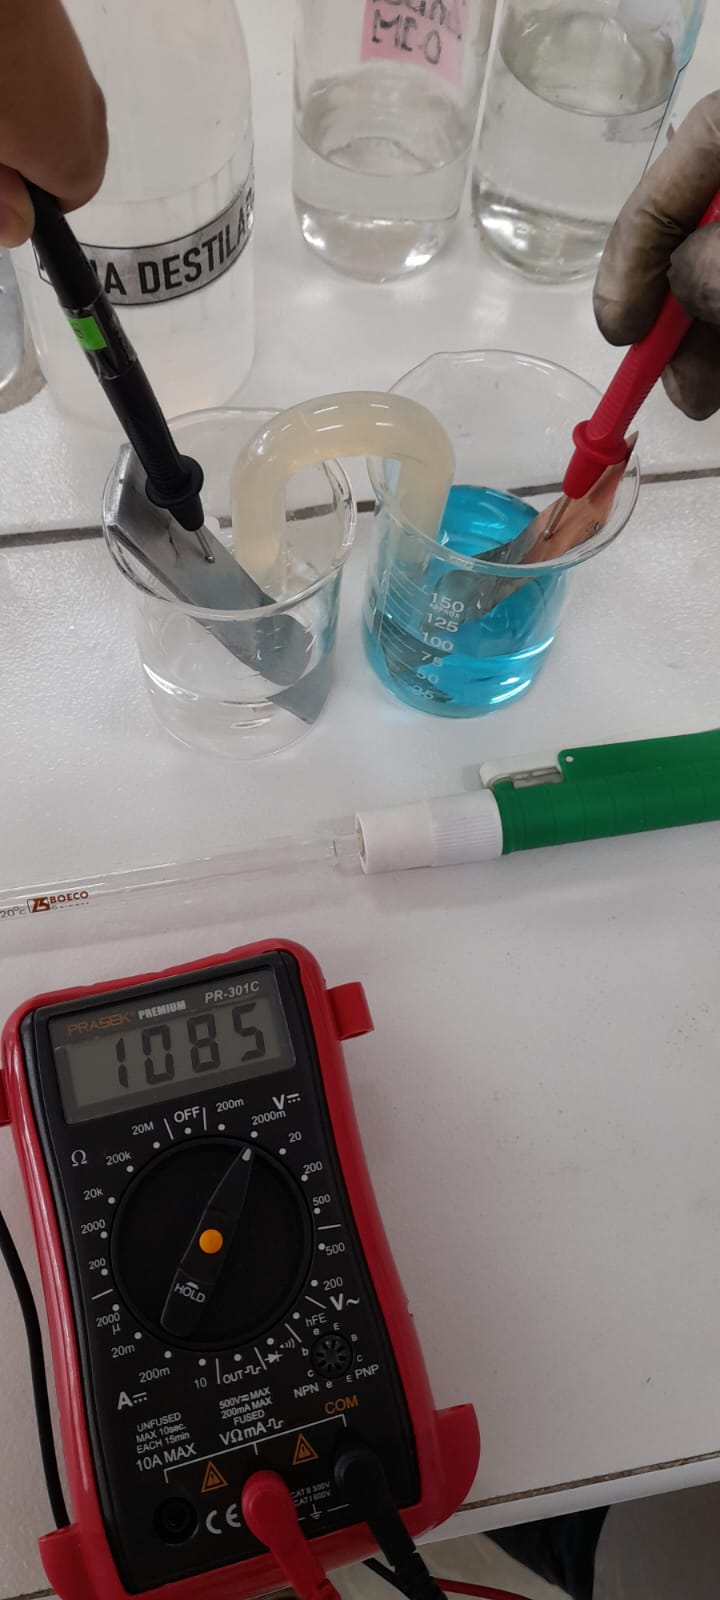
\includegraphics[width=0.25 \textwidth]{Images/01.jpeg}
            \caption{}
        \end{figure}

        \begin{figure}
            \centering
            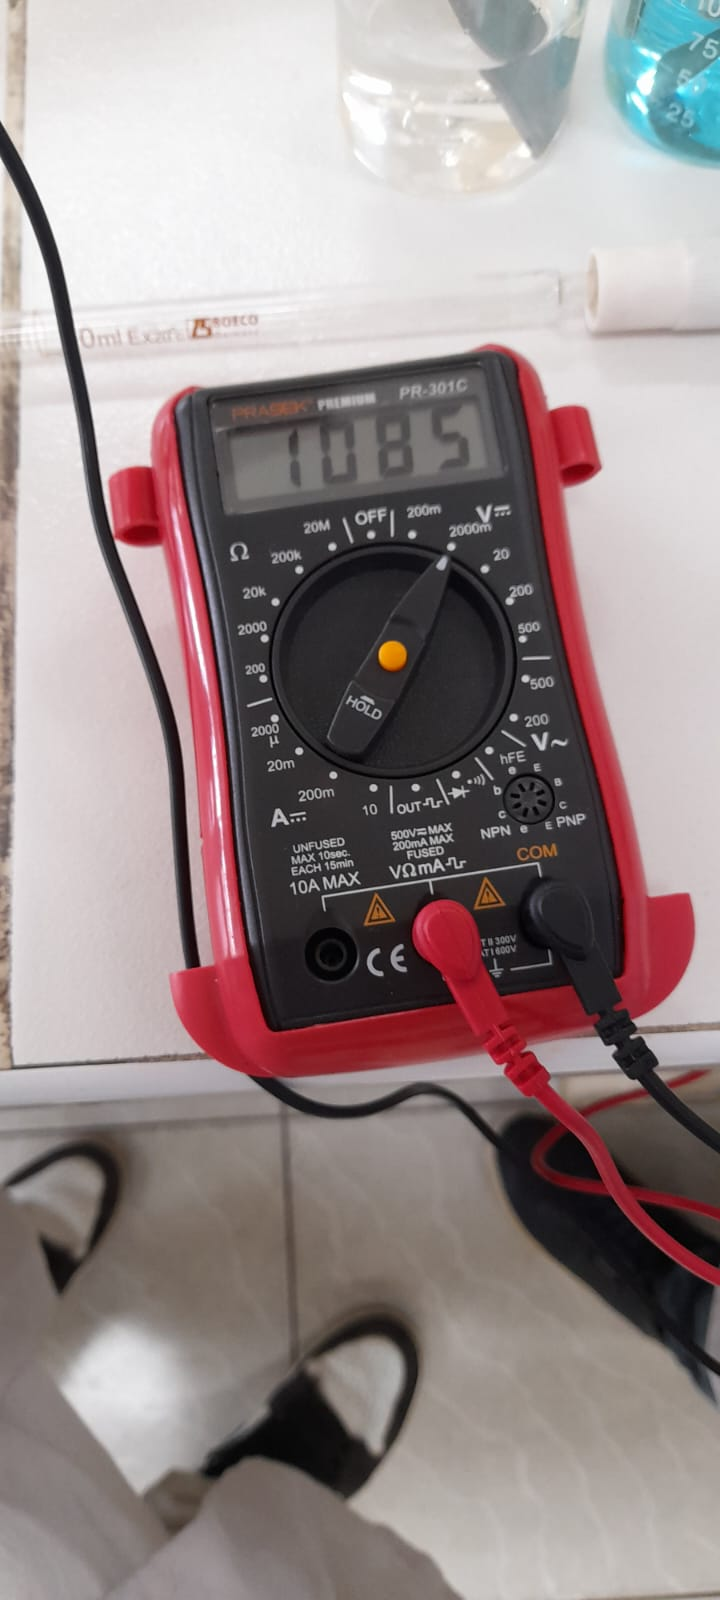
\includegraphics[width=0.25 \textwidth]{Images/02.jpeg}
            \caption{}
        \end{figure}

        \begin{figure}
            \centering
            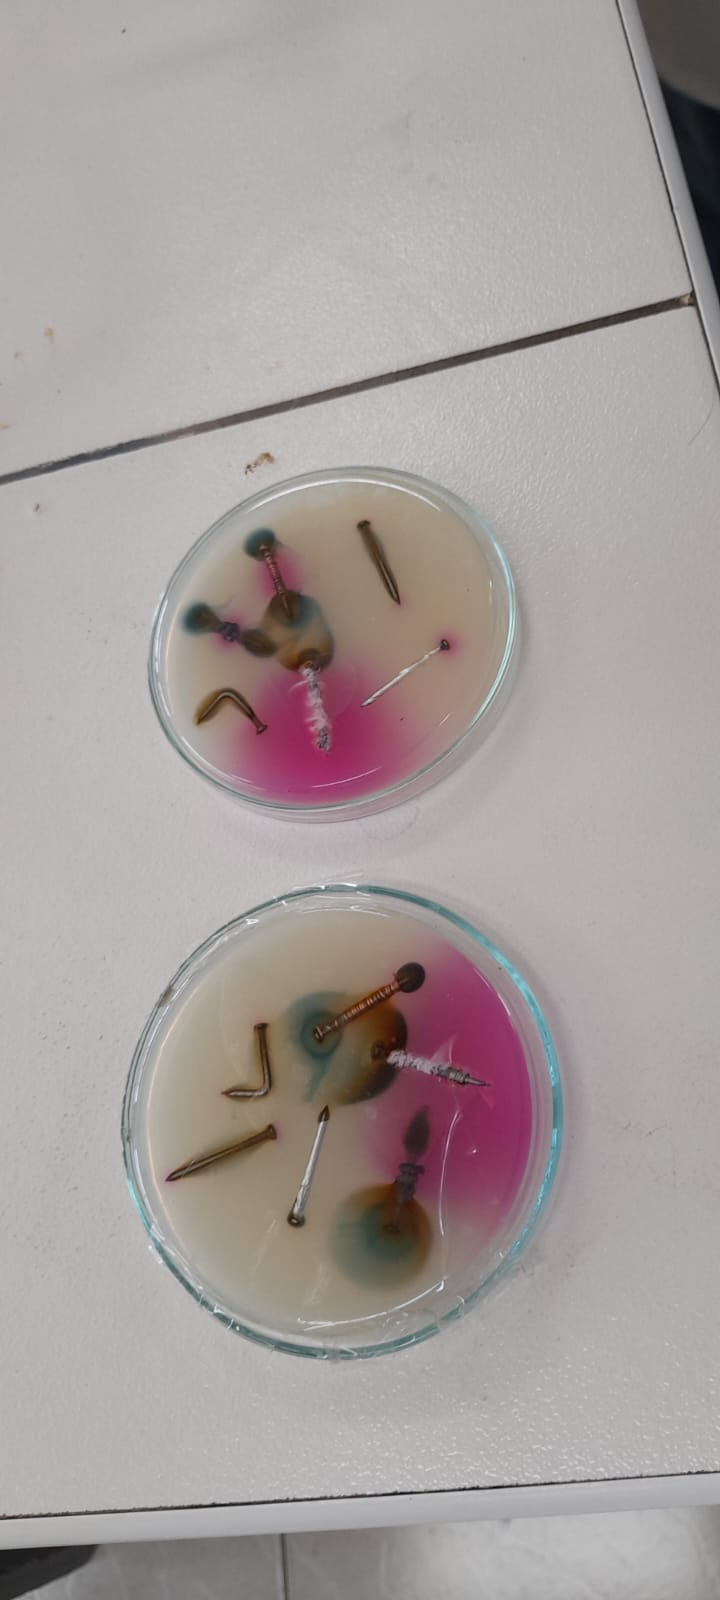
\includegraphics[width=0.25 \textwidth]{Images/03.jpeg}
            \caption{}
        \end{figure}

    \bibliography{bibli}

\end{document}
    
\LaTeX